
\section{Base de datos}

Para poder implementar los servicios de notificaciones push es necesaria una forma de acceder a los
datos que se solicitan en las peticiones de tipo \textit{establish-subscription}. El sistema que 
proporcione estos datos debe cumplir varias condiciones:

\begin{enumerate}
    \item Primero, debe ser capaz de almacenar los datos siguiendo el esquema YANG correspondiente. 
    El lenguaje YANG define una estructura de datos en forma de árbol, definiendo la jerarquía entre
    objetos y pudiéndose codificar en diferentes lenguajes como pueden ser \gls{XML} o \gls{JSON}.
    Por ejemplo el siguiente modelo YANG \ref{COD:EJEMPLOMODELOYANG} se corresponde a los datos \gls{XML}
    listados en el Código \ref{COD:EJEMPLOINSTANCIAYANG}:

    \XMLCode[COD:EJEMPLOMODELOYANG]{Ej. modelo YANG}{Ejemplo de un posible modelo YANG}{ejemplo_yang_1.txt}{}{}{}
   
    \XMLCode[COD:EJEMPLOINSTANCIAYANG]{Instancia modelo YANG en XML}{Una posible instancia del modelo YANG anterior en formato XML}{ejemplo_intancia_yang.xml}{}{}{}

    \item Debe ser compatible con, al menos, el lenguaje de programación utilizado, en este caso,
    Python 3.x, aunque es preferible que exista soporte para otros lenguajes.
    
    \item Debe proporcionar algún mecanismo de notificación de cambios de los datos para poder
    proporcionar notificaciones de tipo \textit{on-change} sin necesidad de hacer \textit{pooling}.
\end{enumerate}

En base a los criterios anteriores se han elegido tres bases de datos candidatas: MongoDB,
Prometheus y Redis. A continuación se van a evaluar cada una de ellas con el fin de elegir la base de datos más adecuada para el proyecto. En el Anexo \ref{appendix:bases_de_datos} se adjunta una tabla comparativa de los tres sistemas.

\subsection{MongoDB}
MongoDB es una base de datos multiplataforma orientada a documentos, clasificada como una base de 
datos NoSQL, que usa el lenguaje BSON, muy similar a JSON en vez del modelo tradicional de las 
bases de datos relacionales donde los datos se almacenan en filas. 

Como podemos ver en la figura~\ref{FIG:MONGO_VS_RDBMS}, las tablas se corresponden a colecciones,
las filas se corresponden a documentos y las columnas se corresponden a campos de los documentos
pero con la ventaja de que MongoDB usa un modelo \textit{schemaless}, por tanto, los campos de los
documentos no son fijos. Dentro de una misma colección cada documento puede tener diferentes campos,
permitiendo la modificación de la estructura de un documento sin tener restricciones impuestas por
la colección (en un RDBMS todas las filas tienen las mismas columnas, es menos flexible). 

% TODO: añadir imágen  de objetos distintos en la misma colección emulando uno de los modelos yang.

\begin{figure}
    [Equivalencias entre MongoDB y RDBMS]
    {FIG:MONGO_VS_RDBMS}
    {Equivalencias entre MongoDB y RDBMS}
    \image{10cm}{}{MongoDB_vs_RMSBD}
\end{figure}

Como ya hemos visto en la introducción de este apéndice, al ser capaz de guardar datos con una
estructura \gls{JSON} es muy idoneo para este proyecto. Además es compatible con muchos lenguajes de
programación como C, CSharp, C++, Go, Java, Javascript, PHP y \textbf{Python}.
\subsection{Prometheus}
Prometheus \cite{prometheus} es una aplicación open-source usada para la monitorización de 
eventos y envío de alertas en tiempo real. Usa base de datos orientada a series temporales, 
dónde cada serie se identifica por un nombre, P.E ``Used Bandwidth \%'', y un conjunto 
de pares clave-valor. Además, cuenta con un potente lenguaje de consultas llamado PromQL que
permite la manipulación de series temporales para la generación de gráficos, tablas y alertas.

Desgraciadamente, este sistema no cumple con varios de nuestros requisitos. En primer lugar,
está optimizado para series temporales mientras que para este proyecto se necesita guardar
instancias de modelos YANG. En segundo lugar, aunque Prometheus dispone de un sistema de alertas
llamado \textit{alertmanager} los tipos de notificaciones de proporciona no se corresponde con las 
necesidades del proyecto. Tal como se ha explicado al principio de esta sección, se necesita un 
mecanismo que detecte cambios en las instancias de los modelos YANG soportados y notificar el 
hilo/proceso que estuviese monitorizando un subárboles determinado de un modelo YANG. Sin embargo,
el \textit{alertmanager} lo que proporciona son alertas basadas en eventos (P.E Temperatura de la 
CPU > 90º durante más de 2 minutos) para administradores de sistemas, ofreciendo diferentes canales
como Slack, Telegram, Correo, SMS, etc. 

\begin{figure}
    [Arquitectura de Prometheus]
    {FIG:PROMETHEUS_ESTRUCTURA}
    {Arquitectura de Prometheus}
    \image{15cm}{}{prometheus_architecture}
\end{figure}

Sin embargo, aunque no sea un sistema adecuado para almacenar los datos de un datastore YANG, se podría estudiar la utilización de Prometheus como sistema de visualización de series temporales que recibiría el cliente a través de notificaciones NETCONF, P.E. el cliente se podría subscribir para recibir la temperatura de la CPU cada 0.5 segundos y se podría utilizar Prometheus para almacenar esa serie temporal y usar sus herramientas de visualización para interpretar los datos 


\subsection{Redis} 
Redsis \cite{redsis_main_page} es un sistema de almacenamiento de datos en memoria de código abierto (licencia BSD) que se utiliza como base de datos, caché y como sistema de envío de mensajes. Admite estructuras de datos como cadenas, hashes, listas, conjuntos, conjuntos ordenados, mapas de bits, indices geoespaciales y flujos. Redis tiene replicación integrada, soporta scripting LUA, transacciones y distintos niveles de persistencia en disco. 

Redis guarda los datos en una estructura de tipo Hashtable como pares clave-valor soportando todos los
tipos de datos ya mencionados. Sin embargo, no permite la existencia de objetos anidados y por tanto no es capaz de representar un objeto YANG de forma completa (solo podría representar un solo nivel).
Además, no existe soporte para la mayoría de tipos de datos que podemos encontrar en las hojas de un modelo YANG como Integer16/32/64, Float y Double.

Redis tiene un sistema de alertas/notificaciones llamado Redis Keyspace Notifications que permite
a clientes subscribirse a canales para recibir notificaciones de eventos que afectan los datos de Redis. 

Sin embargo, debido a las limitaciones de este tipo de almacenamiento, considero que el sistema no es adecuado.

\begin{figure}
    [Estructura de Datos de Redis]
    {FIG:REDIS_ESTRUCTURA}
    {Estructura de Datos de Redis}
    \image{15cm}{}{redis-data-structure-types}
\end{figure}


\subsection{Decisión de diseño}
INCOMPLETO




\section{Virtualizacion}
INCOMPLETO
  \subsection{Maquinas Virtuales}
  INCOMPLETO
  \subsection{Docker}
  INCOMPLETO
  \subsection{Kubernetes}
  INCOMPLETO
\subsection{Decisión de diseño}

% \begin{figure}
%     \centering
%     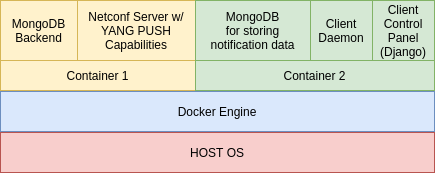
\includegraphics{graphics/docker.png}
%     \caption{Caption}
%     \label{fig:my_label}
% \end{figure}
